\chapter{Analisi Numerica}
\section{Introduzione}
In questo capitolo verranno presentate alcune tecniche per la risoluzione dei
sistemi lineari e il concetto di \textbf{numero di condizionamento}.

Lo sviluppo di un algoritmo di risoluzione di sistemi lineari deve considerare
tre fattori:
\begin{enumerate}
    \item \textbf{Memoria}: l'algoritmo deve richiedere un quantitativo ridotto
          di memoria.
    \item \textbf{Velocità}: l'algoritmo deve essere molto veloce.
    \item \textbf{Precisione}: vogliamo ottenere una soluzione più vicina possibile
          a quella reale.
\end{enumerate}
\subsection{Gestione di Matrici e Vettori}
A livello di programmazione, i vettori possono essere salvati utilizzando
aree congiunte di memoria (array). Mentre, per quanto riguarda le matrici, si
possono salvare in array secondo diverse filosofie:
\begin{itemize}
    \item \textbf{Row Major}: si salvano le righe una dopo l'altra.
          \begin{figure}[!ht]
              \centering
              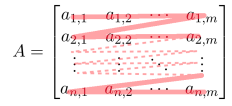
\includegraphics[width=0.25\textwidth]{./img/AnalisiNumerica/RowMajor.png}
              \caption{Esempio di salvataggio di una matrice in Row Major}
          \end{figure}
    \item \textbf{Column Major}: si salvano le colonne una dopo l'altra.
          \begin{figure}[!ht]
              \centering
              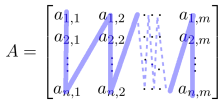
\includegraphics[width=0.25\textwidth]{./img/AnalisiNumerica/ColumnMajor.png}
              \caption{Esempio di salvataggio di una matrice in Column Major}
          \end{figure}
\end{itemize}

Per salvare una matrice \textbf{sparsa} viene sempre salvata come collezione di
tuple $\langle i, \, j,\, val\rangle$. Con questa rappresentazione, anche nota
come \textbf{formato sparso}, ogni qualvolta si effettua un'operazione tra matrici
sparse si trasformano in matrici normali e si applica l'operazione.
\subsection{Gestione Errori}
L'algoritmo creato deve essere valutato in base a quanto è vicino il risultato
restituito rispetto a quello corretto. Questo deve essere fatto in quanto
i risultati sono spesso forniti come numeri floating point e quindi soggetti
a errori di approssimazione.

\begin{definizione}[\textbf{Errore assoluto}]
    Sia $\stackrel{\sim}{\textbf{x}}$ la soluzione approssimata di un sistema
    lineare $A\textbf{x} = \textbf{b}$ e sia $x$ la soluzione corretta, allora
    l'\textbf{errore assoluto} è definito come:
    \begin{equation}
        \epsilon = \|\stackrel{\sim}{\textbf{x}} - \textbf{x}\|
    \end{equation}
    dove $\|\cdot\|$ è una qualsiasi norma fra due vettori.
\end{definizione}
\begin{definizione}[\textbf{Errore relativo}]
    Sia $\stackrel{\sim}{\textbf{x}}$ la soluzione approssimata di un sistema
    lineare $A\textbf{x} = \textbf{b}$ e sia $x$ la soluzione corretta, allora
    l'\textbf{errore relativo} è definito come:
    \begin{equation}
        \epsilon = \frac{\|\stackrel{\sim}{\textbf{x}} - \textbf{x}\|}{\|\textbf{x}\|}
    \end{equation}
    dove $\|\cdot\|$ è una qualsiasi norma fra due vettori.
\end{definizione}

Il problema è conoscere la soluzione esatta del sistema per calcolare l'errore.
Un modo per ottenere la soluzione esatta possiamo inizializzare un vettore $x$ in modo
randomico. In questo modo si calcola il vettore $b =A\cdot x $ e successivamente
si utilizza algoritmo di risoluzione di sistemi per risolvere il seguente
sistema $A\cdot \stackrel{\sim}{x} = b$. In questo modo $x$ è la soluzione esatta
mentre  $\stackrel{\sim}{x}$ è la soluzione approssimata. Ovviamente questa non è
la soluzione reale, ma ci interessa principalmente sapere se è risolvibile il sistema
e con che errore. Questo è determinato dalla matrice $A$ ma non dal vettore dei
termini noti $b$, per questo ci si calcola un vettore $b$ dipendente dalla soluzione
"esatta" randomica.
\begin{teorema}\label{teo:NormeEquivalenti}
    Il comportamento delle norme di vettori in $\mathbb{R}^n$ è equivalente. ossia
    preso un vettore $x\in \mathbb{R}^n$, $\exists c_1,c_2\in \mathbb{R}$ tali che:
    \begin{equation}
        c_1\|x\|_p < \|x\|_q < c_2\|x\|_p
    \end{equation}
\end{teorema}
Il teorema \ref{teo:NormeEquivalenti} ci dice che le norme a meno di alcuni
fattori moltiplicativi restituiscono gli stessi risultati.
\subsection{Velocità}
Come precedentemente detto, un aspetto importante è la velocità dell'algoritmo.
Per calcolare questo parametro dobbiamo contare il numero di operazioni che
effettuiamo, nello specifico si andrà ad utilizzare la complessità asintotica.

Analizziamo ora le velocità delle diverse operazioni:
\begin{itemize}
    \item \textbf{Prodotto Scalare}: sia $(x,y) = \sum_{i=1}^n x_iy_i$ corrisponde
          ad effettuare $n$ prodotti e $n-1$ somme, quindi si ha $n + n - 1 = 2
              n -1 \in \mathcal{O}(n)$
    \item \textbf{Norma di un vettore}: sia $\|x\| = \sqrt{\sum_{i=1}^n x_i^2}$
          corrisponde ad effettuare $n$ prodotti e $n-1$ somme, quindi si ha
          $n + n - 1 = 2n -1 \in \mathcal{O}(n)$
    \item \textbf{Prodotto Matrice-Vettore}: siano $A\in \mathbb{R}^{r\times c}$
          e $v\in \mathbb{R}^c$ allora $Av\in \mathcal{O} (rc) = \mathcal{O}(n^2)$
    \item \textbf{prodotto Matrice-Matrice}: siano $A,B\in \mathbb{R}^{n\times n}$
          allora $AB\in \mathcal{O} (n \cdot n \cdot n) = \mathcal{O} (n^3)$
    \item \textbf{Determinate}: sia $A\in \mathbb{R}^{n\times n}$ allora
          $det(A) \in \mathcal{O}(n!)$.
\end{itemize}
\section{Numero di Condizionamento}
Sappiamo che presa una matrice $A \in \mathbb{R}^{n \times n}$ e un vettore $b
    \in \mathbb{R}^n$ diverso dal vettore nullo, il sistema lineare $A \textbf{x} =
    \textbf{b}$ ammette soluzione se e soltanto se $det(A) \neq 0$.

Purtroppo quando si risolvono i sistemi lineari al calcolatore subentrano una
serie di altri fattori che influenzano il modo in cui si risolve il sistema e,
di conseguenza, la soluzione stessa. Questi fattori sono dovuti essenzialmente
alla rappresentazione dei numeri e agli errori di arrotondamento nelle operazioni.

Oltre a ciò, analizzando le velocità delle operazioni, si può notare che il
calcolo del determinante è molto complesso, quindi non è possibile utilizzarlo
per capire se un sistema è complesso da risolvere.

Per ovviare a questo problema, si introduce il concetto di \textbf{numero di
    condizionamento} calcolato su una matrice. Se tale valore è alto allora il
sistema è complesso da risolvere.
\begin{definizione}[\textbf{Numero di Condizionamento}]
    Presa una matrice $A \in \mathbb{R}^{n \times n}$, il \textbf{numero di
        condizionamento} è definito come:
    \begin{equation}
        cond(A) = \|\lambda_{max}\| \cdot \|\lambda_{min}\|
    \end{equation}
    dove $\lambda_{max}$ e $\lambda_{min}$ sono rispettivamente il massimo e il
    minimo autovalore della matrice $A$ in modulo.
\end{definizione}
Per definizione il numero di condizionamento è una quantità maggiore di $1$.
Vedremo che più questa quantità è vicino a $1$ più il sistema sarà facile da
risolvere numericamente, ossia risente meno dell'algebra di macchina. Di contro
più grande è questa quantità più il sistema sarà risolto “male”.
\begin{esempio}[Numero di Condizionamento di una Matrice di Hillbert]
    Prendiamo una matrice $H \in \mathbb{R}^{n \times n}$ definita nel seguente modo:
    \begin{equation*}
        H_{ij}=\frac{1}{1+i+j}
    \end{equation*}
    Questa matrice è nota con il nome di matrice di Hillbert ed è il classico
    esempio di matrice mal condizionata.
\end{esempio}
\section{Metodi per risolvere i sistemi}
Esistono due tipologie di metodi per la risoluzione dei sistemi lineari:
\begin{itemize}
    \item \textbf{Metodi diretti}: si effettuano delle operazioni per ottenere
          in automatico la soluzione dei sistemi.
    \item \textbf{Metodi iterativi}: sono procedure che creano una sequenza di
          vettori soluzioni che si avvicinano sempre di più alla soluzione esatta
          $\|x -\stackrel{\sim}{x}\|\rightarrow 0$ oppure si calcola $\frac{\|x
                  -\stackrel{\sim}{x}\|}{\|A\stackrel{\sim}{x} - b\|}\rightarrow 0$.
\end{itemize}
\section{Metodi diretti}
Partiamo analizzando il caso più semplice, ovvero che il sistema ammette un unica
soluzione. L'assunzione principale è che le matrici abbiano determinante diverso
da $0$.
\subsection{Sostituzione all'indietro}
Il metodo della \textbf{sostituzione all'indietro} è il metodo più efficiente per
risolvere sistemi composti da una matrice quadrata triangolare superiore.
\begin{equation}
    \begin{cases}
        u_{11}x_1 + u_{12} x_2 + \dots + u_{1n} x_n= b_1 \\
        u_{22}x_2 + u_{23} x_3 + \dots + u_{2n} x_n= b_2 \\
        \vdots                                           \\
        u_{nn}x_n = b_n                                  \\
    \end{cases} \iff \left[\begin{array}{cccc}
            u_{11} & u_{12} & \dots  & u_{1n} \\
            0      & u_{22} & \dots  & u_{2n} \\
            \vdots & \ddots & \ddots & \vdots \\
            0      & \dots  & 0      & u_{nn}
        \end{array} \right] \cdot x = \left[\begin{array}{c}
            b_1    \\
            b_2    \\
            \vdots \\
            b_n
        \end{array}\right]
\end{equation}
A livello computazione è semplice testare se la matrice è compatibile con questo
metodo.

Una volta effettuata la verifica, il metodo coincide con il risolvere il sistema
per sostituzione.
\begin{nota}
    Bisogna stare attenti che la diagonale non contenga $0$ perché ogni volta
    si divide per un termine sulla diagonale.
\end{nota}

Sotto le ipotesi di matrice triangolare superiore possiamo calcolare facilmente
il determinante, basta calcolare il prodotto dei termini sulla diagonale, questo
ci dice che esiste una sola soluzione se il determinante è diverso da $0$
($\mathcal{O}(n)$). In aggiunta, questo ci assicura che la diagonale non contiene $0$.

La complessità dell'algoritmo sarà:
\begin{equation*}
    \#\_righe \cdot \#operazioni\_max\_riga = n \cdot (n - 1 + n - 1 + 1) = n
    \cdot (2n - 1) = \mathcal{O}(n^2)
\end{equation*}
\begin{nota}
    Dove il numero massimo di operazioni per riga è $n - 1$ differenze, $n - 1$
    prodotti e $1$ divisione perché nella prima riga si ha:
    \begin{equation*}
        x_1 = \frac{(b_1 - u_{12} x_2 - u_{13}x_3 - \dots - x_{1n} x_n)}{u_{11}}
    \end{equation*}
\end{nota}
Ogni singola operazione per riga si può ricavare iterativamente nel seguente modo
\begin{equation*}
    x_{n-i} = \frac{(b_i-(u_{n-i},x))}{u_{ii}}
\end{equation*}
Con $x$ inizializzato a tutti $0$ tranne la cella $n$ che sarà inizializzata a:
\begin{equation*}
    x_n = \frac{b_n}{u_{nn}}
\end{equation*}
Mentre $i$ è inizializzato a $1$, ad ogni iterazione si utilizza il vettore $x$
aggiornato nell'iterazione precedente. Al termine si ottiene una soluzione per il
sistema.
\begin{nota}
    Questo metodo può essere utilizzato anche per i sistemi lineari descritti da
    una matrice triangolare inferiore. In questo caso prima sarà necessario
    trasformare la matrice in una matrice triangolare superiore. Questo si può
    fare riordinando le righe della matrice e specchiando la matrice la colonna
    centrale. Lo stesso ragionamento si può applicare anche per matrici diagonali
    rispetto alla antidiagonale.
\end{nota}
\begin{nota}
    Ricorda che quando si effettua un permutazione delle righe il sistema rimane
    invariato, al contrario se effettuassi una permutazione delle colonne allora
    sto cambiando le incognite, perciò dovrei cambiare anche il vettore delle
    incognite se io volessi mantenere lo stesso sistema.
\end{nota}
\subsection{Trasformazioni di Gau$\Beta$}
Per risolvere sistemi a cui sono associate matrici che non sono triangolari,
come quella riportata di seguito, non possiamo più pensare all'algoritmo di
sostituzione all'indietro.
\begin{equation}
    \begin{cases}
        a_{11}x_1 + a_{12} x_2 + \dots + a_{1n} x_n= b_1 \\
        a_{21}x_1 + a_{22} x_2 + \dots + a_{2n} x_n= b_2 \\
        \vdots                                           \\
        a_{n1}x_1 + a_{n2} x_2 + \dots + a_{nn} x_n= b_n \\
    \end{cases}
\end{equation}

Per sistemi generici di $n$ equazioni in $n$ incognite i metodi di risoluzione
sono diversi. L'algoritmo di eliminazione di Gauss si basa sul fatto che, preso
un sistema lineare è possibile modificare le sue equazioni in modo da ottenere
un sistema lineare equivalente, ossia che ha la stessa soluzione del sistema di
partenza. Questo si può fare utilizzando le seguenti trasformazioni:
\begin{itemize}
    \item \textbf{Scambiare le righe}
    \item \textbf{Riduzione}: Sostituire una riga con una combinazione lineare di
          se stessa con un'altra
\end{itemize}
Successivamente si eseguirà sul sistema equivalente il metodo di risoluzione per
sostituzione all'indietro.

Per effettuare riduzione della matrice associata al sistema ad una matrice
triangolare superiore, applichiamo una serie di trasformazioni in modo da azzerare
i coefficienti al di sotto della diagonale. L'applicazioni delle trasformazioni
deve essere effettuata sulle righe della \textbf{augmented matrix form}, ovvero
la matrice del sistema con l'aggiunta del vettore dei termini noti a destra dei
coefficienti delle incognite.
\begin{definizione}[\textbf{Pivot}]
    Il termine che si sceglie per procedere con la sostituzione di tutte le
    equazioni del sistema lineare viene chiamato \textbf{pivot}.
\end{definizione}
\begin{nota}
    Sotto l'ipotesi di sistema risolubile (determinante non nullo) allora il metodo
    di Gau$\Beta$ convergerà ad una matrice triangolare superiore. Quindi non
    rischio di sostituire una riga con un coefficiente moltiplicatore di un'altra
    riga avente denominatore nullo. Quindi, quando abbiamo una riga che ha il
    coefficiente sulla diagonale pari a $0$ allora siamo sicuri che troveremo
    un'altra riga con un coefficiente non nullo.
\end{nota}
\begin{osservazione}
    Durante tutto il procedimento osserviamo che la scelta del pivot e quindi
    del moltiplicatore dipende solamente dalla matrice A e non dal termine noto.
    Il termine noto viene sempre e solo aggiornato in modo da ottenere un sistema
    lineare equivalente!
\end{osservazione}

Calcoliamo ora la complessità di tale algoritmo. Il peggiore dei casi è quando
effettuiamo la prima riduzione. Nello specifico, per essa dobbiamo calcolare:
\begin{equation*}
    R_i = R_i - \frac{a_{11}\cdot a_{a_i1}}{a_{11}} R_1
\end{equation*}
Queste operazioni sono $n + 1$ differenze, $n + 1$ prodotti e $1$ divisione. Quindi
per una riga sono necessarie $1 + n + 1 + n + 1 = 2 n + 3 =\mathcal{O}(n)$.
Questo deve essere ripetuto per $n - 1$ volte per azzerare la prima colonna,
in termini di complessità asintotica $\mathcal{O}(n^2)$. Dal momento che dobbiamo
ridurre un totale di $n-1$ colonne quindi si ha $\mathcal{O}(n^2\cdot n) = \mathcal{O}(n^3)$.
Attualmente non stiamo risolvendo il sistema, bensì lo stiamo solo trasformando,
per anche risolverlo impiegheremo  $\mathcal{O}(n^3+ n^2) =\mathcal{O}(n^3)$.

La scelta su da quale equazione partire porta ad avere cambiamenti sugli errori
ottenuti dal calcolo della soluzione dovuta all'aritmetica floating point. Quindi
l'obiettivo sarà di ridurre al minimo l'errore, sapendo che l'operazione problematica
è la somma/differenza soprattutto quando effettuiamo il calcolo $x + y$ dove $y
    \sim -x$. Quindi possiamo mitigare questi problemi utilizzando il \textbf{pivoting},
ovvero scegliere come pivot quello in valore assoluto maggiore presente sulla
colonna da ridurre.

Esistono due strategie per trovare il miglior pivot:
\begin{itemize}
    \item \textbf{Pivoting Parziale}: si cerca fra i coefficienti della matrice
          nella colonna che vogliamo eliminare il termine che ha il valore
          assoluto più alto.
    \item \textbf{Pivoting Totale}:  si cerca fra tutti i coefficienti della
          sotto matrice il termine più grande in modulo. Una volta scelto il
          coefficiente è necessario fare anche uno scambio di colonne in modo
          tale che quello sia il termine più a destra, altrimenti, andando
          avanti con l'eliminazione di Gau$\beta$, si perderebbe la struttura
          risultante di triangolare superiore.
\end{itemize}

Si sceglie il maggiore perché supponendo di essere in questo esempio:
$$a_{21} - \frac{a_{21}}{a_11} \ a_{22}-\frac{a_{21}}{a_11}$$
Sapendo che $a_{21}=0$ allora sostituisco direttamente con $0$ senza effettuare
la sottrazione (non compiendo errori) e se si sceglie come pivot il massimo allora
$\frac{a_{21}}{a_11}$ sarà piccolo quindi si compie un errore minore nel calcolo
di $a_{22}-\frac{a_{21}}{a_11}$. Si può ottimizzare ancora meglio effettuando il
\textbf{pivoting totale}.
\begin{table}[!ht]
    \centering
    \begin{tabular}{|c|c|c|}
        \hline
        \textbf{Pivot Totale} & \textbf{Casuale} & \textbf{Pivot Più Piccolo} \\
        $3.2138 e^{-14}$      & $1.0214 e^{-12}$ & $6.9658 e^{-11}$           \\
        \hline
    \end{tabular}
\end{table}

Utilizzando il metodo di Gau$\beta$ ha un problema, quando dobbiamo risolvere i
seguenti sistemi che presentano la stessa matrice ma con termini noti diversi:
\begin{equation*}
    Ax=b_1 \quad Ax=b_2 \quad Ax=b_3
\end{equation*}
In questa situazione dobbiamo risolvere tre volte lo stesso sistema in quanto
non si tiene memoria delle operazioni che sono state effettuate.

Sapendo che i termini noti sono indipendenti dalla scelta del pivoting allora
dobbiamo trovare un modo per aggiornare $b_i$ per evitare di aggiornare ogni
volta $A$.
\begin{osservazione}
    Risolvere più volte questo sistema variando $b_i$ coincide con il calcolo
    dell'inversa. Dove $x$ corrisponde alla colonna $i$ dell'inversa con il
    vettore di termini noti $b_i$, dove $b_i$ è il vettore di tutti $0$ tranne
    un $1$ nella posizione $i$-esima.
\end{osservazione}
Per risolvere questo problema uso la decomposizione LU. Ovvero dato un sistema
$Ax=b$, l'idea è di riscrivere la matrice $A$ come il prodotto di $L$ e $U$ ($A
    = L \cdot U$) che rappresentano rispettivamente una matrice triangolare
inferiore e una matrice triangolare superiore. Quindi si risolverà il sistema $L
    \cdot U \cdot x = b$, quando dobbiamo cambiare $b$ basta sostituire $b$ e le
matrici $L$ e $U$ rimarranno uguali.

Per risolvere $L\cdot U \cdot x =b$, prima si risolve $L\cdot y =b$ con una
\textbf{soluzione in avanti} $\mathcal{O}(n^2)$, poi si risolve $U \cdot x = y$
con una \textbf{soluzione all'indietro} $\mathcal{O}(n^2)$.
\begin{teorema}
    Sia $A \in \mathbb{R}^{n\times n}$ una matrice non singolare (determinante
    non nullo), allora esistono $L,U \in \mathbb{R}^{n\times n}$ tali che $A =
        L \cdot U$.
    Dove la matrice $U$ è definita come:
    \begin{equation*}
        U=\left[\begin{array}{ccc}
                a_{11} & a_{12}  & a_{13}   \\
                0      & a_{22}' & a_{23}'  \\
                0      & 0       & a_{33}'' \\
            \end{array}\right]
    \end{equation*}
    Mentre la matrice $L$ è definita come:
    \begin{equation*}
        L=\left[\begin{array}{ccc}
                1      & 0      & 0 \\
                l_{21} & 1      & 0 \\
                l_{31} & l_{32} & 1 \\
            \end{array}\right]
    \end{equation*}
\end{teorema}
Per calcolare $L,U$ ci si impiega $\mathcal{O}(n^3)$ e generalmente $L$ viene
salvata in $U$.
\begin{nota}
    Possiamo pensare di risolvere $Ax=b$ in $x= A^{-1}b$, il problema è che per
    trovare $A^{-1}$ servono $\mathcal{0}(n^4)$ operazioni in cui si accumulano
    errori. Inoltre per trovare l'inversa risolviamo più sistemi.
\end{nota}
\begin{nota}
    Un possibile utilizzo della decomposizione $LU$ è quello di calcolare il
    determinante della matrice $A$. Questo può essere fatto nel seguente modo:
    \begin{equation}
        det(A) = det(LU) = det(L)det(U)
    \end{equation}
    dal momento che $L$ e $U$ sono matrici triangolari, allora il determinante è
    il prodotto dei coefficienti sulla diagonale. Inoltre $L$ ha solamente il
    valore $1$ sulla diagonale, quindi $det(L) = 1$ mentre il $det(U) = u_{11}
        \dots u_{nn}$. Quindi per calcolare il determinante costa $\mathcal{O}(n^3)$
    dalla decomposizione.
\end{nota}

\subsection{Decomposizione PALU}
La decomposizione PALU permette di risolvere un insieme di sistemi lineari in
cui varia solamente il termine noto.
\begin{teorema}
    Sia $A \in \mathbb{R}^{n\times n}$ una matrice quadrata tale che $det(A) \neq 0$,
    allora esistono tre matrici $P,L,U$ tali che:
    \begin{equation}
        PA=LU
    \end{equation}
    dove $P$ è una matrice di permutazione, $L$ è una matrice triangolare inferiore
    con diagonale unitaria e $U$ è una matrice triangolare superiore.
\end{teorema}
La matrice di permutazione $P$ mi permette di effettuare la scelta del pivot migliore.
\begin{nota}
    Anche per la decomposizione $PALU$, il determinante è semplice calcolare
    il determinante della matrice $A$, nel seguente modo:
    \begin{equation*}
        det(PA) = det(LU)
    \end{equation*}
    quindi $det(P) \cdot det(A) = det(L) \cdot det(U)$, dal momento che $P$ è
    una matrice di permutazione allora si può dimostrare che il determinante della
    matrice di permutazione si può calcolare come:
    \begin{equation*}
        det(P) = (-1)^{\#\_scambi}
    \end{equation*}
    Quindi $(-1)^{\#\_scambi}det(A) = det(L)det(U)$ ovvero:
    \begin{equation*}
        det(A) = \frac{det(L)det(U)}{(-1)^{\#\_scambi}}
    \end{equation*}
\end{nota}
\subsection{Decomposizione di Cholesky}
Se la matrice $A$ che stiamo considerando, presenta delle caratteristiche
particolari, può essere fattorizzata utilizzando una strategia differente
rispetto alla decomposizione $PALU$, ovvero la decomposizione di \textbf{Cholesky}.

Si può applicare questa decomposizione su matrici che rispettano queste ipotesi:
\begin{itemize}
    \item $A$ simmetrica, $A = A^t$.
    \item $A$ è definita positiva, $y^t A y >0, \forall y \in \mathbb{R}, y \neq \vec{0}$,
          oppure tutti i suoi autovalori sono positivi (non si ammettono
          autovalori nulli).
\end{itemize}
\begin{teorema}
    Sia $A \in \mathbb{R}^{n\times n}$ una matrice simmetrica e definita positiva,
    allora esiste una matrice $R \in \mathbb{R}^{n\times n}$ tale che:
    \begin{equation}
        A = R^t R
    \end{equation}
\end{teorema}
La matrice $R$ è una matrice triangolare superiore.
\begin{dimostrazione}
    Dimostreremo questo teorema in modo costruttivo, ossia diremo come costruire
    la sola matrice $R$ che ci serve a partire dai coefficienti della matrice $A$.

    Data la matrice $A$ definita come:
    \begin{equation*}
        A=\left[\begin{array}{cccc}
                a_{11} & a_{12} & \dots  & a_{1n} \\
                a_{21} & a_{22} & \dots  & a_{2n} \\
                \vdots & \vdots & \ddots & \vdots \\
                a_{n1} & a_{n2} & \dots  & a_{nn} \\
            \end{array}\right]
    \end{equation*}
    che rispetta le ipotesi della decomposizione di Cholesky, supponiamo di
    suddividere la matrice in queste regioni.
    \begin{equation*}
        A=\left[\begin{array}{c|c}
                \alpha       & \textbf{a}_1^t \\
                \textbf{a}_1 & A_\ast         \\
            \end{array}\right]
    \end{equation*}
    dove abbiamo definito:
    \begin{equation*}
        \textbf{a}_1 = \left[\begin{array}{c}
                a_{12} \\
                \vdots \\
                a_{1n} \\
            \end{array}\right] \quad A_{1, 1} = \left[
            \begin{array}{ccc}
                a_{2, 2} & \dots  & a_{2, n} \\
                \dots    & \vdots & \dots    \\
                a_{n, 2} & \dots  & a_{n, n}
            \end{array} \right]
    \end{equation*}
    In questo modo dobbiamo cercare i coefficienti della matrice $R$ che permetta
    di ricavare ciascun coefficiente della matrice $A$ che si sta selezionando.

    Quindi la matrice $R$ può essere definita come:
    \begin{equation*}
        A=\left[\begin{array}{c|c}
                \rho          & \underline{r} \\
                \hline
                \underline{0} & R_\ast        \\
            \end{array}\right]
    \end{equation*}
    In questo modo bisogna trovare $\rho, r$ che permetta di ottenere secondo la
    relazione $A = R^tR$ il coefficiente $a_{11}$, successivamente si reitera lo
    stesso procedimento per tutti gli altri coefficienti ottenendo sotto-matrice
    $R_\ast$.

    Data la matrice $A$, la quale rispetta le ipotesi della decomposizione, allora
    sapendo che essa è simmetrica possiamo rappresentarla come segue:
    \begin{equation*}
        A=\left[\begin{array}{c|ccc}
                a_{11}            & \underline{a_1} \\
                \hline
                \underline{a_1}^t & A_\ast
            \end{array}\right]
    \end{equation*}
    Quindi possiamo dire che:
    \begin{equation*}
        \left[\begin{array}{c|ccc}
                a_{11}            & \underline{a_1} \\
                \hline
                \underline{a_1}^t & A_\ast
            \end{array}\right] = A = R^tR= \left[\begin{array}{c|c}
                \rho            & \underline{0}^t \\
                \hline
                \underline{r}^t & R_\ast^t        \\
            \end{array}\right]\left[\begin{array}{c|c}
                \rho          & \underline{r} \\
                \hline
                \underline{0} & R_\ast        \\
            \end{array}\right]=\left[\begin{array}{c|c}
                \rho^2                   & \rho \cdot\underline{r}                      \\
                \hline
                \underline{r}^t\cdot\rho & \underline{r}^t\underline{r}+R_\ast^t R_\ast \\
            \end{array}\right]
    \end{equation*}
    Dato che il vettore $r \in \mathbb{R}^n$ allora possiamo dire che:
    \begin{equation*}
        \underline{r}^t\underline{r} \in \mathbb{R}^{n\times n}
    \end{equation*}
    Dalla generazione del prodotto $R^tR$ allora possiamo dire che:
    \begin{equation*}
        \begin{cases}
            \rho^2 = a_{11}                                                                     \\
            \underline{r} = \rho \underline{a}_1 & \text{che vale sia per riga sia per colonna} \\
            \underline{r}^t\underline{r}+R_\ast^t R_\ast = A_\ast
        \end{cases}
    \end{equation*}
    Risolvendo questo sistema le incognite $\rho, r, R_\ast$:
    \begin{equation*}
        \begin{cases}
            a_{11} = \rho ^2                    \\
            \underline{a}_1= \rho \underline{r} \\
            A_\ast = \underline{r}^t\underline{r}+R_\ast^t R_\ast
        \end{cases}\iff \begin{cases}
            \rho = +\sqrt{a_{11}}                \\
            \underline{r}= \rho  \underline{a}_1 \\
            R_\ast^t R_\ast = A_\ast - \frac{1}{a_{11}} \underline{a}_1^t \underline{a}_1
        \end{cases}
    \end{equation*}
    Dato che una delle ipotesi su cui si basa la decomposizione di Cholesky è che la
    matrice sia definita positiva, allora siamo sicuri ogni coefficiente sulla
    diagonale sarà sempre $> 0$, permettendoci di calcolare $\rho$.
\end{dimostrazione}

Questo sistema è ricorsivo e il problema è che bisogna reiterare il procedimento
per ottenere gli altri coefficienti, quindi è necessario che $R_\ast ^t R_\ast$
sia simmetrica e definita positiva. Proviamo a dimostrarlo, chiamiamo $B$ la
matrice definita come $R_\ast ^t R_\ast$, quindi $B = A_\ast - \frac{1}{a_{11}}
    \underline{a}_1^t \underline{a}_1$.
\begin{itemize}
    \item Dimostriamo che la matrice B sia simmetrica:
          \begin{equation*}
              B^t = \left(A_\ast - \frac{1}{a_{11}} \underline{a}_1^t
              \underline{a}_1\right)^t= A_\ast - \frac{1}{a_{11}} (\underline{a}_1^t
              \underline{a}_1)^t =A_\ast - \frac{1}{a_{11}} \underline{a}_1^t
              \underline{a}_1 = B
          \end{equation*}
    \item Dimostriamo che sia definita positiva:
          \begin{equation*}
              0<\underline{y}^t A \underline{y} = \left[\begin{array}{cc}
                      \eta & \underline{y_1}
                  \end{array}\right]\left[\begin{array}{c|ccc}
                      a_{11}            & \underline{a_1} \\
                      \hline
                      \underline{a_1}^t & A_\ast
                  \end{array}\right]\left[\begin{array}{c}
                      \eta \\
                      \underline{y_1}
                  \end{array}\right] = \left[\begin{array}{cc}
                      \eta & \underline{y_1}
                  \end{array}\right]\left[\begin{array}{c}
                      \eta a_{11}+\underline{a_1}\underline{y}_1^t \\
                      \eta\underline{a_1}^t + A_\ast \underline{y}_1^t
                  \end{array}\right] =
          \end{equation*}
          \begin{equation*}
              = \eta^2 a_{11}+\eta\underline{a_1}\underline{y}_1^t+\eta
              \underline{y}_1\underline{a_1}^t + \underline{y}_1 A_\ast
              \underline{y}_1^t = \eta^2 a_{11}+2\eta\underline{a_1}\underline{y}_1^t +
              \underline{y}_1 A_\ast \underline{y}_1^t>0
          \end{equation*}
          Quindi equivale ad una disequazione di secondo grado in $\eta$, quindi
          bisogna controllare che $\Delta < 0\implies b^2-4ac<0$, questo significa:
          \begin{equation*}
              \Delta =(2\underline{a_1}\underline{y}_1^t)^2 -4a_{11}
              \underline{y}_1 A_\ast \underline{y}_1^t = \not 4(\underline{a_1}
              \underline{y}_1^t)^2 -\not 4 a_{11} \underline{y}_1 A_\ast \underline{y}_1^t
              < 0\iff
          \end{equation*}
          \begin{equation*}
              \iff \underline{y}_1 A_\ast \underline{y}_1^t - \frac{1}{a_{11}}
              (\underline{a_1}\underline{y}_1^t)^2>0
          \end{equation*}
          Ma ripetendo la matrice $B$ e per controllare che sia definita positiva
          è esattamente:
          \begin{equation*}
              \underline{y}B\underline{y}^t=\underline{y}A_\ast\underline{y}^t -
              \frac{1}{a_{11}} \underline{y}\underline{a}_1^t \underline{a}_1\underline{y}^t >0
          \end{equation*}
          Che è esattamente quanto trovato precedentemente.
\end{itemize}

\subsection{Perturbazione dei dati}
Per ora sono stati introdotti solo dei metodi diretti per risolvere in modo approssimato 
sistemi di equazione lineare. Ora vogliamo studia come la soluzione trovata cambia
al variare dei coefficienti di $A$ e $b$ del sistema.

Fissiamo $A$ e consideriamo i seguenti sistemi lineari
\begin{equation*}
    Ax=b \ \ \ \ \ \ Ax = b+ \delta b
\end{equation*}
In modo tale che $\|\delta b\| < b$. Sia $\stackrel{\sim }{x}$ la soluzione del 
sistema $Ax=b$, vogliamo scoprire come $\stackrel{\sim}{x}$ si modifica nel sistema 
perturbato. Possiamo osservare innanzitutto
$$A\stackrel{\sim}{x}=b \implies \|A\stackrel{\sim}{x}\|=\|b\|\implies 
\|A\|\|\stackrel{\sim}{x}\|\ge \|b\|\implies\frac{1}{\|\stackrel{\sim}{x}\|}\le \frac{\|A\|}{\|b\|}$$
Con quanto detto, dal momento che $\stackrel{\sim}{x}$ è una soluzione del sistema 
allora $det(A)\ne 0 $ quindi la matrice è invertibile, di conseguenza
$$Ax = b+\delta b\implies A^{-1}Ax = A^{-1}(b+\delta b)\implies A^{-1}Ax = A^{-1}b+A^{-1}\delta b$$ 
Dal momento che per un sistema in cui esiste una soluzione allora si ha che $x= A^{-1}b$
allora possiamo dire che 
$$A^{-1}Ax = A^{-1}b+A^{-1}\delta b\implies x = \stackrel{\sim}{x}+A^{-1}\delta b\implies x - \stackrel{\sim}{x} = A^{-1}\delta b$$
Anche qui possiamo passare alle norme
$$\|x - \stackrel{\sim}{x} \|= \|A^{-1}\delta b\|$$
utilizzando le proprietà delle norme si ha
$$\|x - \stackrel{\sim}{x} \|\le\|A^{-1}\|\|\delta b\|$$

Ora unendo le due due relazioni tra le soluzioni e i singoli sistemi, ovvero 
a sinistra si moltiplicano le norme delle soluzioni e a destra si moltiplicano 
le norme dei termini dei sistemi.

$$\|\frac{1}{\stackrel{\sim}{x}}\|\|x - \stackrel{\sim}{x} \|\le   \frac{\|A\|}{\|b\|} \|A^{-1}\|\|\delta b\|$$
Questo vale per una qualsiasi norma, fissiamo la norma $2$, allora possiamo introdurre 
il \textbf{numero di condizionamento}.
$$\frac{\|x - \stackrel{\sim}{x} \|}{\|\stackrel{\sim}{x}\|}\le   \frac{\|A\|}{\|b\|} \|A^{-1}\|\|\delta b\|\implies
\frac{\|x - \stackrel{\sim}{x} \|}{\|\stackrel{\sim}{x}\|}\le   \|A\| \|A^{-1}\|\frac{\|\delta b\|}{\|b\|}\implies 
\frac{\|x - \stackrel{\sim}{x} \|}{\|\stackrel{\sim}{x}\|}\le   \|A\| \|A^{-1}\|\frac{\|\delta b\|}{\|b\|}\implies $$

\section{Metodi iterativi}
Dato un generico sistema $Ax=b$ con $A$ invertibile.
I metodi iterativi partono da un vettore iniziale $x^{(0)}$, creano una sequenza 
di soluzioni $x^{(k)}$ che si avvicinano sempre di più alla soluzione esatta 
$\stackrel{\sim}{x}$.

\subsection{Fill-in}
Dal momento che la maggior parte delle volte sono molto grandi e spesso sparse 
allora verranno salvate secondo la rappresentazione sparsa. 

Nel momento in cui si effettua una decomposizione PALU o Cholesky è possibile che 
le matrici risultanti non siano sparse, questo fenomeno è chiamato \textbf{fill-in}.
Questo comporta che per una matrice sparsa, una volta applicata una decomposizione,
essa potrebbe essere soggetta a fenomeno di \textbf{fill-in} quindi produce 
delle matrici non sparse, comportando un aumento di complessità spaziale portanto 
ad occupare troppa memoria. I metodi iterativi permettono di risolvere questo problema,
perché utilizzando le operazioni tra matrici, preservano la natura sparsa quindi 
non si incombe nel fenomeno di fill-in.

\subsection{Criterio di arresto}
Come detto in precedenza, i metodi iterativi continuano a generare soluzioni sempre 
più vicine a quella esatta. 
Negli algoritmi iterativi si ha una quantità, chiamata \textbf{tolleranza}, che
coincide con la soglia che specifica quando terminare le iterazioni. Si termina 
quando vale la seguente relazione
$$\frac{\|x^{(k)}-\stackrel{\sim}{x}\|}{\|\stackrel{\sim}{x}\|} < \texttt{tolleranza}$$

Non potendo conoscere la soluzione esatta allora si riscrive la relazione utilizzano i seguenti metodi 
di arresto:
\begin{itemize}
    \item \textbf{incremento tra due iterate}: alla iterazione $k$ si calcola
    $$\frac{\|x^{(k)}-x^{(k-1)}\|}{\|x^{(0)}\|}< \texttt{tolleranza}$$
    Questo misura quanto le quantità $x^{(k)}$ e $x^{(k-1)}$ differiscono. Ci si 
    ferma quando la differenza è minima. Quindi questo corrisponde a calcolare l'errore relativo rispetto alla soluzione 
    precedente normalizzato rispetto la soluzione iniziale.
    \item \textbf{residuo scalato}: alla iterazione $k$ si calcola
    $$\frac{\|b- Ax^{(k)}\|}{\|b\|}< \texttt{tolleranza}$$
    Dove $A$ e $b$ sono la matrice e il vettore dei termini noti del sistema che 
    si sta risolvendo. Quindi questo corrisponde a calcolare l'errore relativo rispetto alla soluzione 
    precedente normalizzato rispetto la soluzione iniziale.
    
\end{itemize}

 della soluzione $k$-esima
normalizzato secondo la la prima soluzione o secondo il vettore dei termini noti.

\begin{nota}
    Questi criteri funzionano per qualsiasi norma si vuole utilizzare.
\end{nota}

Analizzando la \textbf{complessità del criterio di arresto basato sull'incremento tra due 
iterate successive}, si può notare che si effettua una sottrazione tra vettori 
di dimensione $n$ ($n$ somme ovvero $\mathcal{O}(n)$), la norma ha una complessità
di $\mathcal{O}(n)$ (quindi $2\mathcal{O}(n)$ perché si calcola due volte) e 
successivamente si ha $1$ divisione.
Il costo totale risulta
$$\mathcal{O}(n^2)+ \mathcal{O}(n)+2\mathcal{O}(n)+1 = \mathcal{O}(n)$$

Per quanto riguarda la \textbf{complessità del criterio di arresto basato sull'incremento tra due 
iterate successive} si hanno delle operazioni più complesse:
\begin{itemize}
    \item prodotto tra matrice e vettore: $\mathcal{O}(n^2)$
    \item somma tra vettori: $\mathcal{O}(n)$
    \item calcolo di due norme: $2\mathcal{O}(n)$
    \item un rapporto: $\mathcal{O}(1)$
\end{itemize}
Il totale risulta 
$$\mathcal{O}(n^2)+ \mathcal{O}(n)+2\mathcal{O}(n)+1 = \mathcal{O}(n^2)$$

Il costo è maggiore rispetto al primo criterio anche se rimane sempre polinomiale 
di grado basso. In aggiunta si può notare che spesso i metodi iterativi calcolano
già la quantità $b-Ax^{(k)}$ per ottenere la soluzione $x^{(k+1)}$, quindi la parte 
più onerosa del calcolo del residuo si sposta nel calcolo della soluzione successiva.

\begin{nota}
    Quando si calcola il residuo si calcola una sola volta la norma di $b$, perché
    per tutto l'algoritmo il vettore rimane invariato.
\end{nota}

\begin{nota}
    In aggiunta non è stato tenuto conto che quando calcoliamo i criteri di arresto
    quando facciamo il prodotto matrice-vettore, la matrice è sparsa, quindi 
    il prodotto non è $\mathcal{O}(n^2)$ ma una complessità dipendente dalle entrate 
    non nulle.
\end{nota}

\subsection{Generico algoritmo iterativo}
Tutti gli algoritmi iterativi sono identici a meno della metodologia di calcolo
della soluzione $x^{(k)}$.

Un generico algoritmo prende in input:
\begin{itemize}
    \item una matrice $A$
    \item un vettore dei termini noti $b$
    \item una tolleranza \texttt{tolleranza}
    \item eventuali parametri addizionali utili per il calcolo della soluzione 
    $k$-esima.
\end{itemize}

Il vettore $x^{(0)}$ di partenza e sotto opportune ipotesi della matrice $A$, la 
scelta della soluzione iniziale mantiene invariata la convergenza dell'algoritmo.

Si ha un ciclo while che ha come condizione la verifica del criterio di arresto,
ovvero uno dei criteri specificati precedentemente. Oltre al criterio di arresto 
spesso si aggiunge un numero di iterazioni massime perché spesso si rischia di 
non poter mai raggiungere la soluzione esatta.

Nell'algoritmo non si effettuano mai operazioni che modificano la matrice $A$,
quindi non si rischierà l'effetto fill-in.

\begin{nota}
    Il numero di iterazioni massime, per alcuni problemi, può essere stabilito
    a priori in base alla dimensione della matrice. In generale si considera
    sempre un numero arbitrariamente alto
\end{nota}

% TODO: aggiungere l'algoritmo inb pseudocodice



\subsection{Metodi iterativi stazionari}
Per definire un metodo risolutivo iterativo, si inizia da una procedura di \textbf{splitting}.
Data una matrice $A\in \mathbb{R}^{n\times n}$, supponiamo di spezzarla nel seguente 
modo
$$A=P-N$$
con $P,N\in \mathbb{R}^{n\times n}$. Con questa decomposizione il sistema lineare 
si riscrive in
$$Ax= b \iff (P-N)x= b \iff Px = Nx+b \iff x= P^{-1}Nx+P^{-1}b$$
L'ultima uguaglianza suggerisce la procedura iterativa, ovvero partendo da una 
soluzione iniziale $x^{(0)}$ si ha
\begin{equation}
    x^{k+1} =  P^{-1}Nx^{k}+P^{-1}b
    \label{eq:iterativo_stazionario}
\end{equation}

Tutti i metodi iterartivi si basano sul fatto che il calcolo della matrice $P^{-1}$ 
sia veloce e facile. Se non fosse così allora converrebbe trovare l'inversa di 
$A$ al posto di $P$, in modo tale da calcolare $x=A^{-1}b$.

Questi metodi vengono chiamati stazionari perché le matrici $P,N$ non dipendono 
dal parametro $k$.

\begin{teorema}
    Supponiamo che esista una decomposizione di $A=P-N $ in due matrici $P, N$ simmetriche 
    e definite positive. Se anche la matrice $2P-N$ è definita positiva allora 
    il metodo iterativo definito nell'equazione \ref{eq:iterativo_stazionario} 
    converge per ogni valore iniziale $x^{(0)}$ e $|\lambda_{\max}| < 1$.

    Dove $\lambda_{\max}$ è l'autovalore di modulo massimo della matrice $P^{-1}N$.
    Inoltre la convergenza è monotona rispetto alle norme $\|\cdot\|_p$
\end{teorema}
